\documentclass[border=5pt]{standalone}
\usepackage{tikz}
\usetikzlibrary{arrows.meta, positioning}
\usepackage{xcolor}

% Brand colors
\definecolor{Garnet}{HTML}{73000A}
\definecolor{NinetyBlack}{HTML}{363636}
\definecolor{SeventyBlack}{HTML}{5C5C5C}
\definecolor{FiftyBlack}{HTML}{A2A2A2}
\definecolor{TenBlack}{HTML}{ECECEC}
\definecolor{Atlantic}{HTML}{466A9F}

\begin{document}
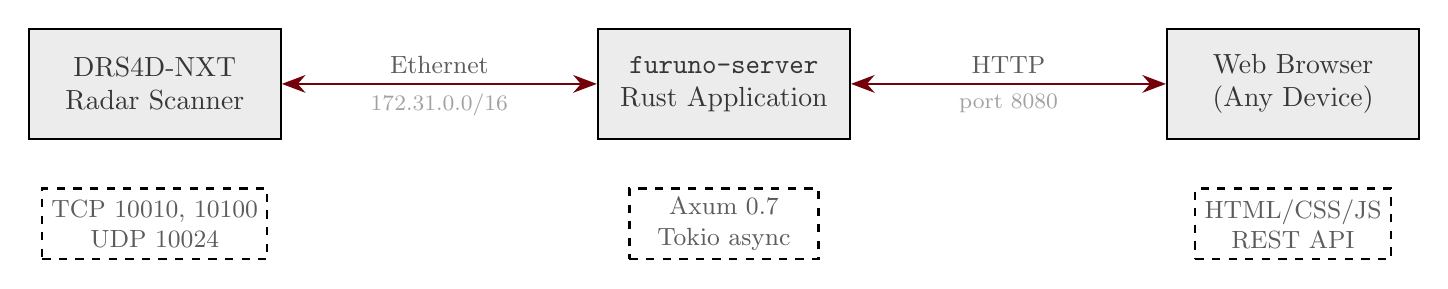
\begin{tikzpicture}[
    block/.style={draw, thick, minimum width=3.2cm, minimum height=1.4cm, align=center, fill=TenBlack, text=NinetyBlack},
    netblock/.style={draw, thick, dashed, minimum width=2.4cm, minimum height=0.9cm, align=center, fill=white, text=SeventyBlack, font=\small},
    arr/.style={-{Stealth[length=3mm]}, thick, Garnet},
    darr/.style={{Stealth[length=3mm]}-{Stealth[length=3mm]}, thick, Garnet},
]
    \node[block] (radar) {DRS4D-NXT\\Radar Scanner};
    \node[block, right=4cm of radar] (server) {\texttt{furuno-server}\\Rust Application};
    \node[block, right=4cm of server] (browser) {Web Browser\\(Any Device)};

    \draw[darr] (radar) -- node[above, font=\small, text=SeventyBlack] {Ethernet} node[below, font=\footnotesize, text=FiftyBlack] {172.31.0.0/16} (server);
    \draw[darr] (server) -- node[above, font=\small, text=SeventyBlack] {HTTP} node[below, font=\footnotesize, text=FiftyBlack] {port 8080} (browser);

    \node[netblock, below=0.6cm of radar] {TCP 10010, 10100\\UDP 10024};
    \node[netblock, below=0.6cm of server] {Axum 0.7\\Tokio async};
    \node[netblock, below=0.6cm of browser] {HTML/CSS/JS\\REST API};
\end{tikzpicture}
\end{document}
